Ideally, the score assigned by the model to a decoy should not depend
on its position and orientation.  To allow the model to learn this
invariance, the rotational and translational degrees of freedom of all
decoy structures are randomly sampled during the training.
%
Figure~\ref{Fig:DecoysScoreDistribution} shows the distributions of
scores for several decoy structures of the same target (T0832),
calculated for 900 rotations and translations sampled uniformly.
While the score of a given structure is not strictly invariant under
rotation and translation, it has a relatively narrow, unimodal
distribution.  More importantly, the difference between the average
scores of two decoys is usually larger than their variances. To reduce
the influence of the choice of rotation and translation on the final
ranking, we estimate the score of each decoy from the average of 90
scores calculated for random rotations and translations.

\begin{figure}[H]
    \centering
    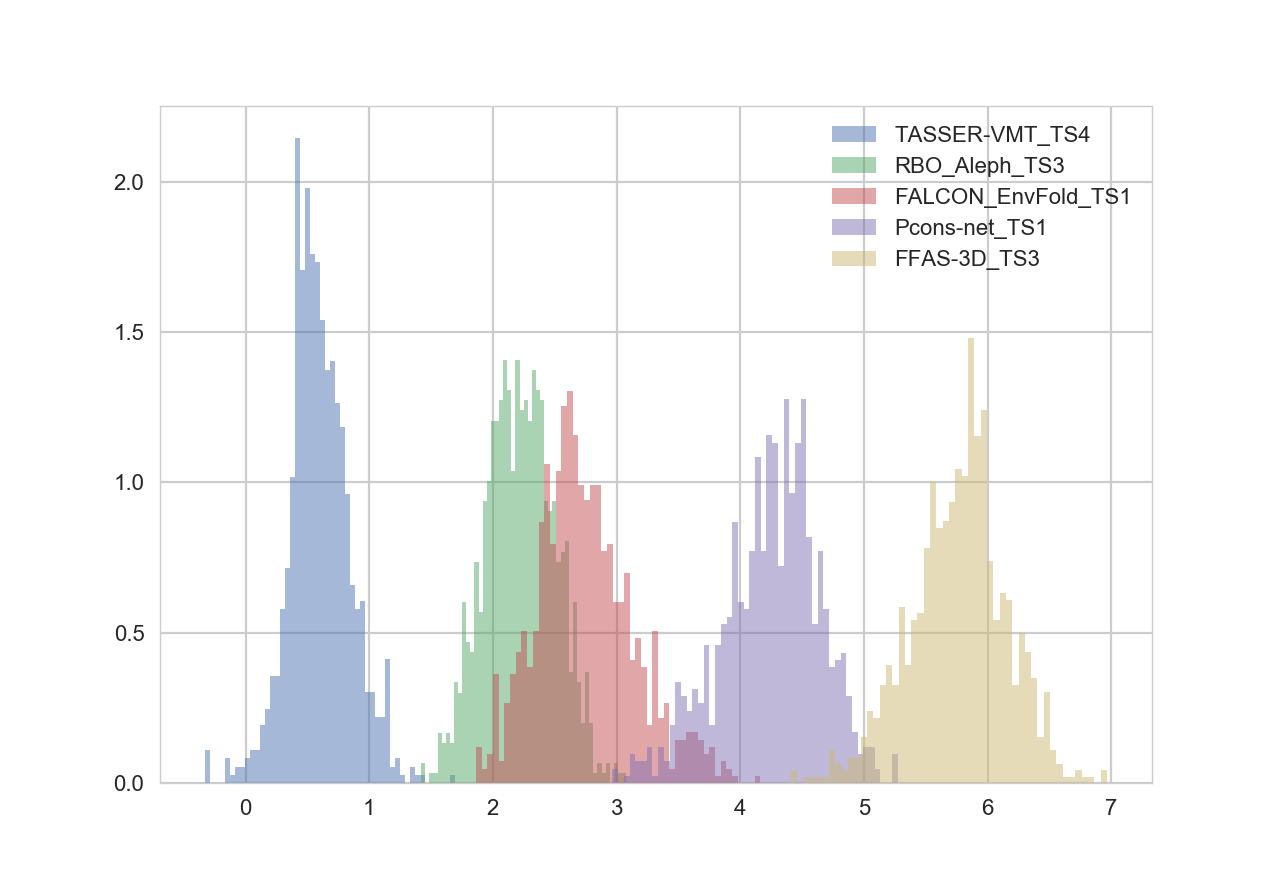
\includegraphics[width=\linewidth]{Fig/decoys_sampling_dist.eps}
%
    \caption{Distributions of the $f$ scores of five decoys for target
    T0832 under random translations and rotations. A lower score
    represents a higher quality.}
%
    \label{Fig:DecoysScoreDistribution}
\end{figure}

Table~\ref{Tbl:TestResults} shows a comparison of our model (3DCNN)
with state-of-the-art model quality assessement methods: ProQ2D,
ProQ3D~\cite{uziela2017proq3d}, VoroMQA~\cite{olechnovivc2017voromqa},
and RWplus~\cite{zhang2010novel}.
%
ProQ2D uses carefully tuned features based on surface area
accessibilities, residue-residue contacts, predicted and observed
seconday structure, residue conservation and atomic contacts. ProQ3D
employs the same features as ProQ2D, as well as some Rosetta energy
terms \ref{leaverfay2011rosetta}. For both ProQ2D and ProQ3D, the
features are used as input for a deep neural network to predict both
the local and global quality of the structure.
%
VoroMQA uses knowledge-based potentials that depend on the contact
surface between every pair of heavy atoms in the protein (or the
solvent).
%%% GL: The next sentence is detail.
%%The contact surfaces are calculated by representing atoms as spheres
%%with the radii equal to the van der Waals radii of the corresponding
%%atoms and using Voronoi tesselation to obtain the contact surface.
%
RWplus uses a pairwise knowledge-based potential that uses
freely-joined chain model to calculate distance distributions in the
reference state.
%%% GL: ??? This is not clear.


%%% GL: Use this paragraph to create some expectations from the
%%% reader. Note that I'm not framing the paragraph in terms of the
%%% reasons why we pick each model but in terms of what is
%%% interesting/good about each one.
ProQ2D and ProQ3D methods are derived from ProQ2, the best-performing
single-model algorithm in CASP11, and are expected to perform better
than the original ProQ2 and ProQ3 methods.
%
RWplus is a representative of the widespread knowledge-based approach
to separating the native structure from its decoys, such as
DOPE \ref{???}  or DFIRE \ref{???}.
%%% GL: It's important to cite these because they are the better known
%%% methods. See the DOPE and DFIRE references in the RWplus
%%% reference.
%
VoroMQA uses an approach distinct from both the common
machine-learning techniques exemplified by the ``ProQ'' methods and
the knowledge-based potential techniques exemplified by the RWplus
method.
%
Moreover, these methods have available source codes or executables.
This allows us to re-evaluate their performance on our CASP11
benchmark, for which the decoys side chains are optimized using
SCWRL4.

%%% GL: Try to put this into another paragraph. It doesn't work as a
%%% standalone paragraph.
Targets T0797, T0798, T0825 are removed from this benchmark because
they were released for multimeric prediction.

\begin{table}[H]
\begin{center}
\begin{tabular}{ c | c | c | c | c }
    MQA method & Loss & Pearson $R$ & Spearmann $\rho$ & Kendall $\tau$ \\ \hline
    \multicolumn{5}{ c }{Stage 1} \\ \hline
    ProQ3D   &0.046 &0.755 &0.673 &0.529 \\
    ProQ2D   &0.064 &0.729 &0.604 &0.468 \\
    \textbf{3DCNN} &0.064 &0.535 &0.425 &0.325 \\    
    VoroMQA  &0.087 &0.637 &0.521 &0.394 \\
    RWplus   &0.122 &0.512 &0.402 &0.303 \\ \hline
    
    \multicolumn{5}{ c }{Stage 2} \\ \hline
    VoroMQA  &0.063 &0.457 &0.449 &0.321 \\ 
    \textbf{3DCNN} &0.064 &0.421 &0.409 &0.288 \\
    ProQ3D   &0.066 &0.452 &0.433 &0.307 \\
    ProQ2D   &0.072 &0.437 &0.422 &0.299 \\
    RWplus   &0.089 &0.206 &0.248 &0.176 \\ \hline

\end{tabular}
%
    \caption{Performance comparison of our method (3DCNN) with other
    state-of-the-art model quality assessment methods on the CASP11
    dataset stages~1 and 2 (see text). The table reports the absolute,
    per-target average values of the correlation coefficients.}
    \label{Tbl:TestResults}
\end{center}
\end{table}

